\infolevone{
\chapter[Introduction]{Introduction
\footnote{Authors: X. YYY \email(xxx@jlab.org)}
}
}
    
\infolevone{
Hall~C is one of the three experimental areas at JLab. This manual
attempts to describe the experimental equipment that makes up this facility
and to provide instructions for the safe and effective use of this equipment.
In this operations manual safety is addressed in the sense that proven
procedures are provided. Potential hazards associated with the operation
of each piece of equipment and responsible personnel are listed for each
end station subsystem in the Experiment Safety Assessment Document
for Hall C Base Equipment 
(the \htmladdnormallinkfoot{ESAD}{http://www.jlab.org/Hall-C/document}).  

\section{General Issues}

There are a number of potentially hazardous systems which are required
at any accelerator complex.
In this section we outline the extent to which these general site hazards
affect the operation of experiments in Hall~C and list those which
require special training. For more information on site safety systems
and regulations the user is referred to the JLab EH\&S Manual.

The principal contacts for the JLab EH\&S group are:

\begin{itemize}
\item[~]Bert Manzlak  - x7556
\item[~]Charles Hightower - x7608
\end{itemize}

\subsection{Oxygen Deficiency Hazard}

Because of the presence of cryogens (for the super conducting magnets
of the HMS, the M\o ller polarimeter and for cooling the cryogenic
targets) Hall~C is listed as an Oxygen Deficiency Hazard (ODH) area of
Class 0 (with the exception of the area above the crane railing which
is ODH-2).  This rating requires that those wishing to have unescorted
access to the hall must take the JLab ODH training course once every
two calender years. This course is typically taught once monthly by a
representative of the EH\&S group.  Further, those working above the
crane railing must have more extensive ODH training as documented in
the JLab EH\&S manual.

There are ODH sensors in the hall which automatically trigger audible
alarms and blue lights. The alarms sound and the lights will flash if
an ODH condition is detected.

Aside from the more or less global concerns about rapidly expanding
cryogenic gases displacing the air there is another
way in which one could encounter an ODH situation in connection with Hall~C
operations. The problem is that of work in confined spaces where
the atmospheric composition may be different from that of the hall at
large. Examples of such spaces are the main spectrometer vacuum vessel,
which is evacuated during normal use (and is usually brought back to ambient
pressure by filling it with dry nitrogen gas), the HMS gas Cerenkov detector
which is normally filled with an oxygen-free gas mixture, and the
SOS gas Cerenkov detector. Before work can be done in any of the
above areas the oxygen content of the atmosphere in the closed vessel should
be verified by EH\&S personnel.

\subsection{Radiation Safety and the Personnel Safety System }

JLab's high intensity, high energy electron beam is a potentially lethal
radiation source and hence many redundant measures
aimed at preventing accidental exposure of personnel to the beam are in place.
This is the purpose of the Personnel Safety System.

The current status of Hall~C is displayed in the Hall~C counting house
on a sign with red lighted letters. The possible conditions are:
\begin{description}
\item[Beam Permit] There is potentially beam in the hall.
\item[Power Permit] In this mode all devices which normally prevent beam 
transport to Hall may be removed or energized.  This is one level below 
that required for beam delivery.
No personnel are allowed in the hall when it is at this level.
\item[Sweep] The machine safety officers are securing the hall.
No access is permitted during this process.
\item[Controlled Access] Access is permitted only by using the keyed
interlock system (A procedure for this type of entry is listed below).
\item[Restricted Access] The entry gate to the hall is open and trained
personnel with appropriate dosimetry may enter.
\end{description}

If the hall is in either Beam Permit or Power Permit states it is impossible
for personnel to enter. If a situation arises that requires a hall entry
then the shift leader will call the Machine Control Center (MCC) and
request an entry. The state of Hall~C will then be lowered to
controlled access and a limited number of trained personnel can enter
the hall via the two door entry gate from the labyrinth. It
is required that personnel entering have a  Radiation Dosimeter
and they must have completed the radiation worker safety training
course at JLab or another DOE laboratory and JLab specific Radiation Worker
Training.

Access to Hall~C is allowed under a General Radiation Work Permit (GRWP).  The 
GRWP specifies access requirements for areas within the Hall.  For instance, access to the 
detector huts or spectrometer carriage may be allowed before a general area radiation 
survey is completed, but access to the target chamber platform may not be allowed 
without a radiation dose rate survey and contamination control survey.  As such, access to 
the target chamber platform may require a specific RWP (SRWP); this would be identified 
in the GRWP.  Each individual must read and sign the GRWP posted in the Counting 
House before entering the hall.

The controlled access procedure is as follows.
\begin{enumerate}

\item{Access to Hall~C is allowed under a General  Radiation Work Permit (GRWP). The GRWP  specifies access requirements for areas within the Hall. For instance, access to the detector huts or spectrometer carriage may be allowed before a general area radiation survey is completed but access to the target chamber platform may not be allowed without a radiation dose rate survey and contamination control survey.}

\item{The hall status sign in the counting house must
read ``controlled access." If not the shift leader must call the MCC
and they will send a radiation survey team over to check the
radiation levels in the hall.}

\item{Proceed downstairs to the entry gate to the hall
and call the MCC at 7050 {\bf before touching the door}. Inform the
MCC crew chief of your name and the names of those accompanying you
and request that they open the outer door.}

\item{Hang up the phone and enter the gate area. The last
person in should close the outer door after entering the gate area.}

\item{Each person entering must take a key from the key bank
and inform the MCC via the phone or intercom which key they have taken.
The keys form a personnel accounting system and all the keys must
be in the bank for the hall to be returned to a beam permit state.
Therefore one should {\bf NEVER} leave the downstairs with a key.
In addition to the individual keys there is a master key which
must be removed from the key bank and placed in the master lock. This
is normally done by the radiation officials who survey the hall.}

\item{The MCC will need to see that all personnel entering have
a JLab radiation dosimeter. They verify this visually with a TV camera in the gate area.
Do not open the inner, hall side, gate door at this time and
it is {\bf never permissable for both gate doors to be open 
simultaneously}.}

\item{After everyone has a key the inner door will be opened
allowing entry into the tunnel leading to Hall~C.
The inner door {\bf must be shut} behind the last person entering.}

\item{When the work in the hall is complete you must
either push the buzzer button by the inner door or call the
MCC to get back into the gate area.
The keys should be returned to the bank and the last person leaving
must remove the master key from
the master lock and replace it in the first position of the
bank (This key is normally placed in the master position by the individual who
first surveys the hall when it is opened for a controlled access).}

\end{enumerate}

While downstairs the status of the beam is visible on the yellow
run-safe boxes. The lights should either be green or yellow.
{\bf If the run-safe box in an area where you are working has a red
light lit you should hit the scram button immediately.}

If the hall status reads restricted access then there is free
access for trained personnel.

\subsubsection{Induced Activity}

In addition to the hazard of direct exposure to the electron beam you must
be aware of the potential for induced radioactivity in objects near the path
of the beam.  The GRWP specifies the requirements for hall entry after beam shutdown.  
Typically, a radiation susrvey is done to evaluate conditions in the hall.  If radiation levels 
exceed certain thresholds, then specific signs, postings, and barriers will be installed by the 
RCG or ARMs.  In addition, verbal instructions may be given to personnel in the area 
regarding access to various locations.  If it is necessary to remove or modify beam line or 
target chamber components, or to perform any work in a posted Radiation Area, you must 
consult the RCG before beginning work.  In many cases a specific RWP (SRWP) is 
required for work.  SRWPs for many activities will be available in the Counting House for 
review.  Any item which was in the hall during beam delivery and needs to be removed 
from the hall, must be surveyed by the RCG prior to removal.  All hardware, materials, or 
components which are waste items should be placed in the large blue drums available for 
potentially activated material.  The RCG will survey these items before disposal. 

If it becomes necessary to perform work on any piece of equipment in the hall
that may have received a significant dose of direct radiation {\bf you
must have it surveyed by a radiation monitor before} you work can begin.
This mean's that all work on beamline or target chamber equipment will
involve a radiation survey.

If it is necessary to remove any item from the hall after or during a running
period it should be surveyed first. {\bf All components must be surveyed
and released by a radiation officer before they can be removed from the hall}.

\subsubsection{Radiation Control Personnel}

The radiation safety group at JLab includes the following personnel:

\begin{center}
\begin{tabular}{llll}
\hline
Name  & Extension & Pager & Home Phone \\
\hline
Bob May & 7632 & 680-7632 & 424-5525 \\
Dan Dotson & 7296 & 680-7296 & 1-804-693-9590 \\
David Hamlette & 7219 & 680-7219 & 766-3827 \\
Earl Ratliff & 7118 & 680-1682 & 1-804-642-1832 \\
George Walker & 7417 & 680-7417 & 1-804-693-5146 \\
Keith Welch & 7212 & 680-7212 & 875-1707 \\
Melvin Washington & 6243 & 680-6243 & 599-0241 \\
Scott Schwahn & 7551 & 680-7551 & 564-1957 \\
Zach Edwards & 	7147 & 680-7147 & 872-7519 \\
\hline
\end{tabular}
\end{center}


\subsection{AC Power}

The sections below describe a)~the AC power distribution system installed
in Hall~C, and b)~procedures to follow in the event of a power failure
(either planned or unplanned).

\subsubsection{AC Power Distribution System}

There are basically three voltages of AC power service available in Hall~C.
These are three phase 208 Volt power, three phase 480 Volt power and
single phase 120 Volt power. There are two different types of 120 Volt
service available, regular and ``clean" power. The clean power
should be used for noise sensitive applications such as power supplies
for detectors etc. It is not permissable to power machinery from
the clean power. If you are uncertain about the use of AC power in any given
situation ask the shift leader or any Hall~C staff member.

The AC power is really three different systems.

\begin{enumerate}
\item{AC power for the air conditioning system, fans, and the
outer perimeter of the hall (i.e. the outlets). This power is
supplied from a transformer which is isolated from the power
used for instrumentation.}
\item{AC power (1800 Amps) for power supplies and instrumentation
on the spectrometer. This power is distributed to various panels
(all marked), and supplies power for all pumps etc.}
\item{AC clean power
\begin{itemize}
\item{fed from separate transformer which is interlocked to the
VESDA systems.}
\item{only supplies power to detectors in the huts of HMS and SOS.}
\item{also supplies power to racks near magnet power supplies (except
racks 5-9).}
\end{itemize}}
\end{enumerate}

For specifics of the AC power, see the printout of electrical drawings
WBS6. The full list is included as  Figures~\ref{fig:elect_dwgs1}--\ref{fig:elect_dwgs3}.
\clearpage
\begin{figure}
\begin{center}
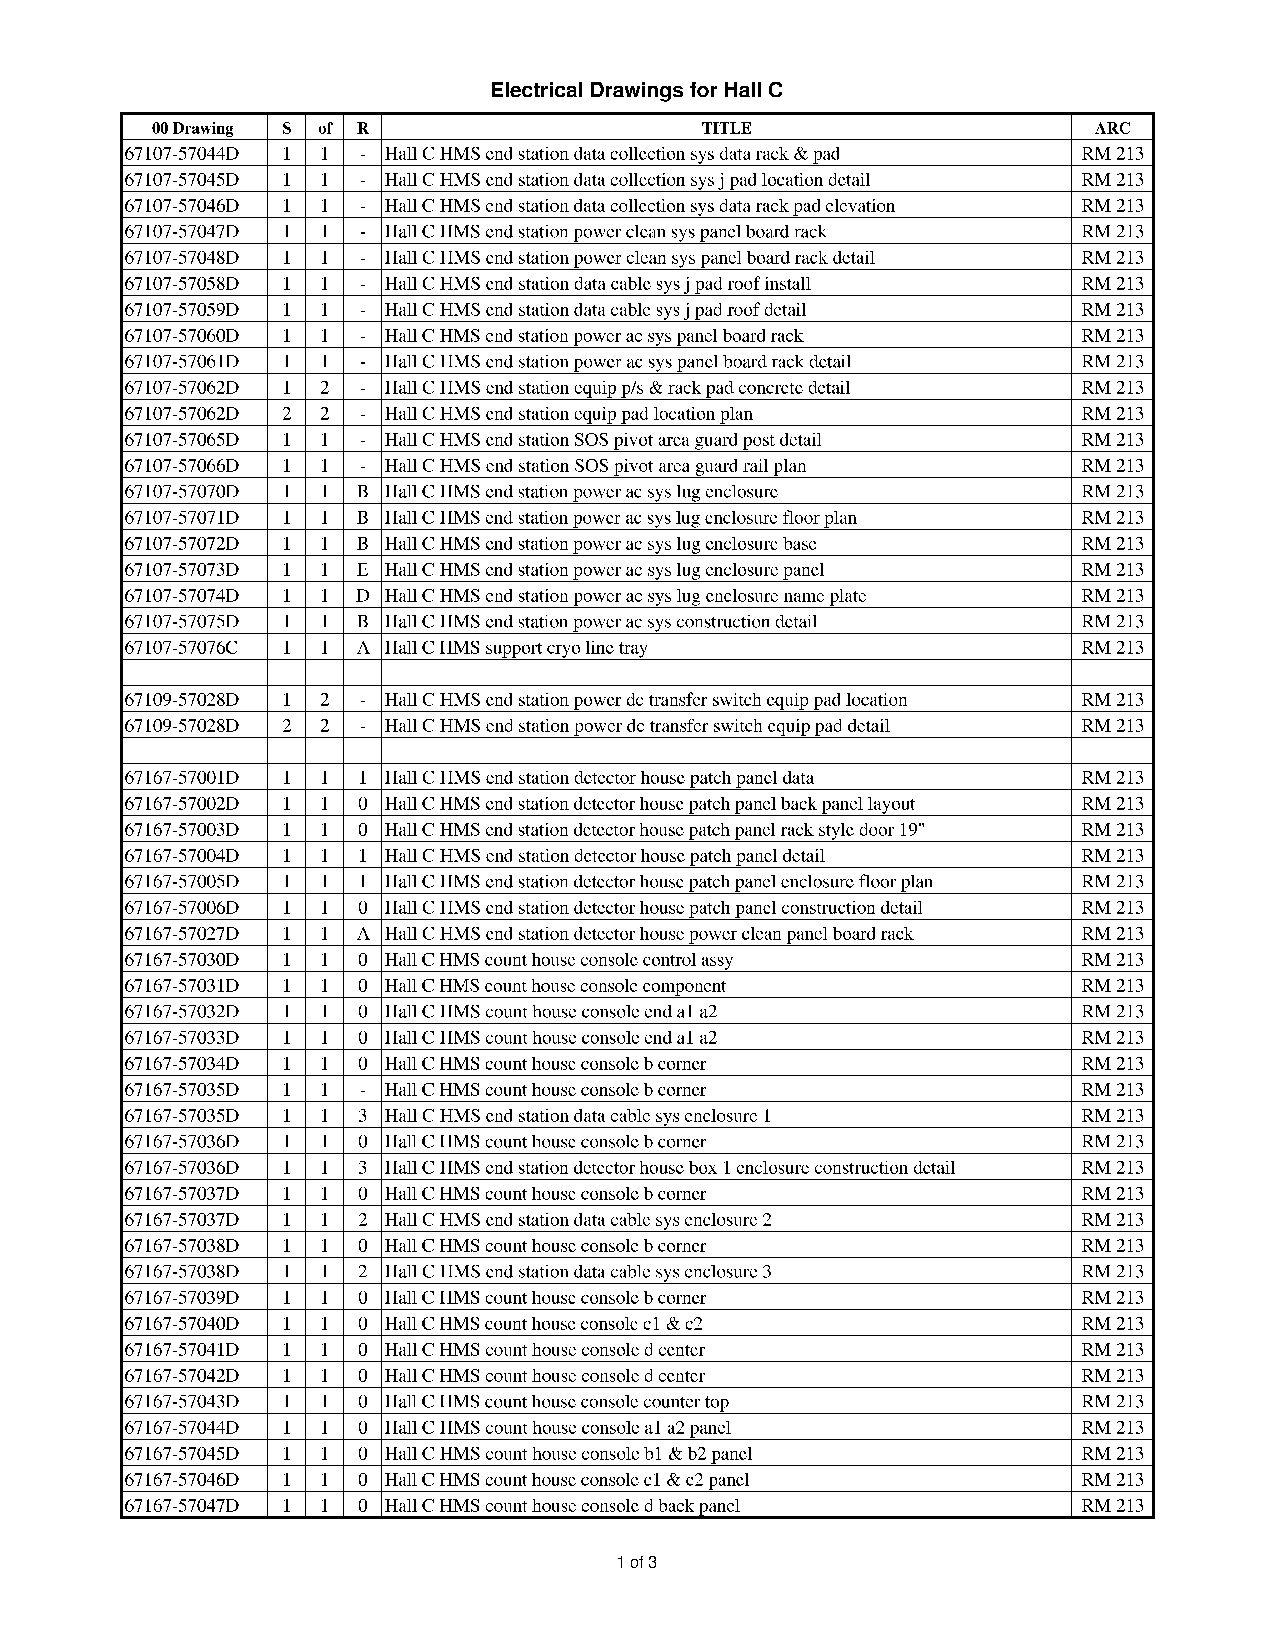
\includegraphics[height=7in]{ele1p.pdf}
\caption{Electrical Drawings for Hall~C (1 of 3)}
\label{fig:elect_dwgs1}
\end{center}
\end{figure}

\clearpage
\begin{figure}
\begin{center}
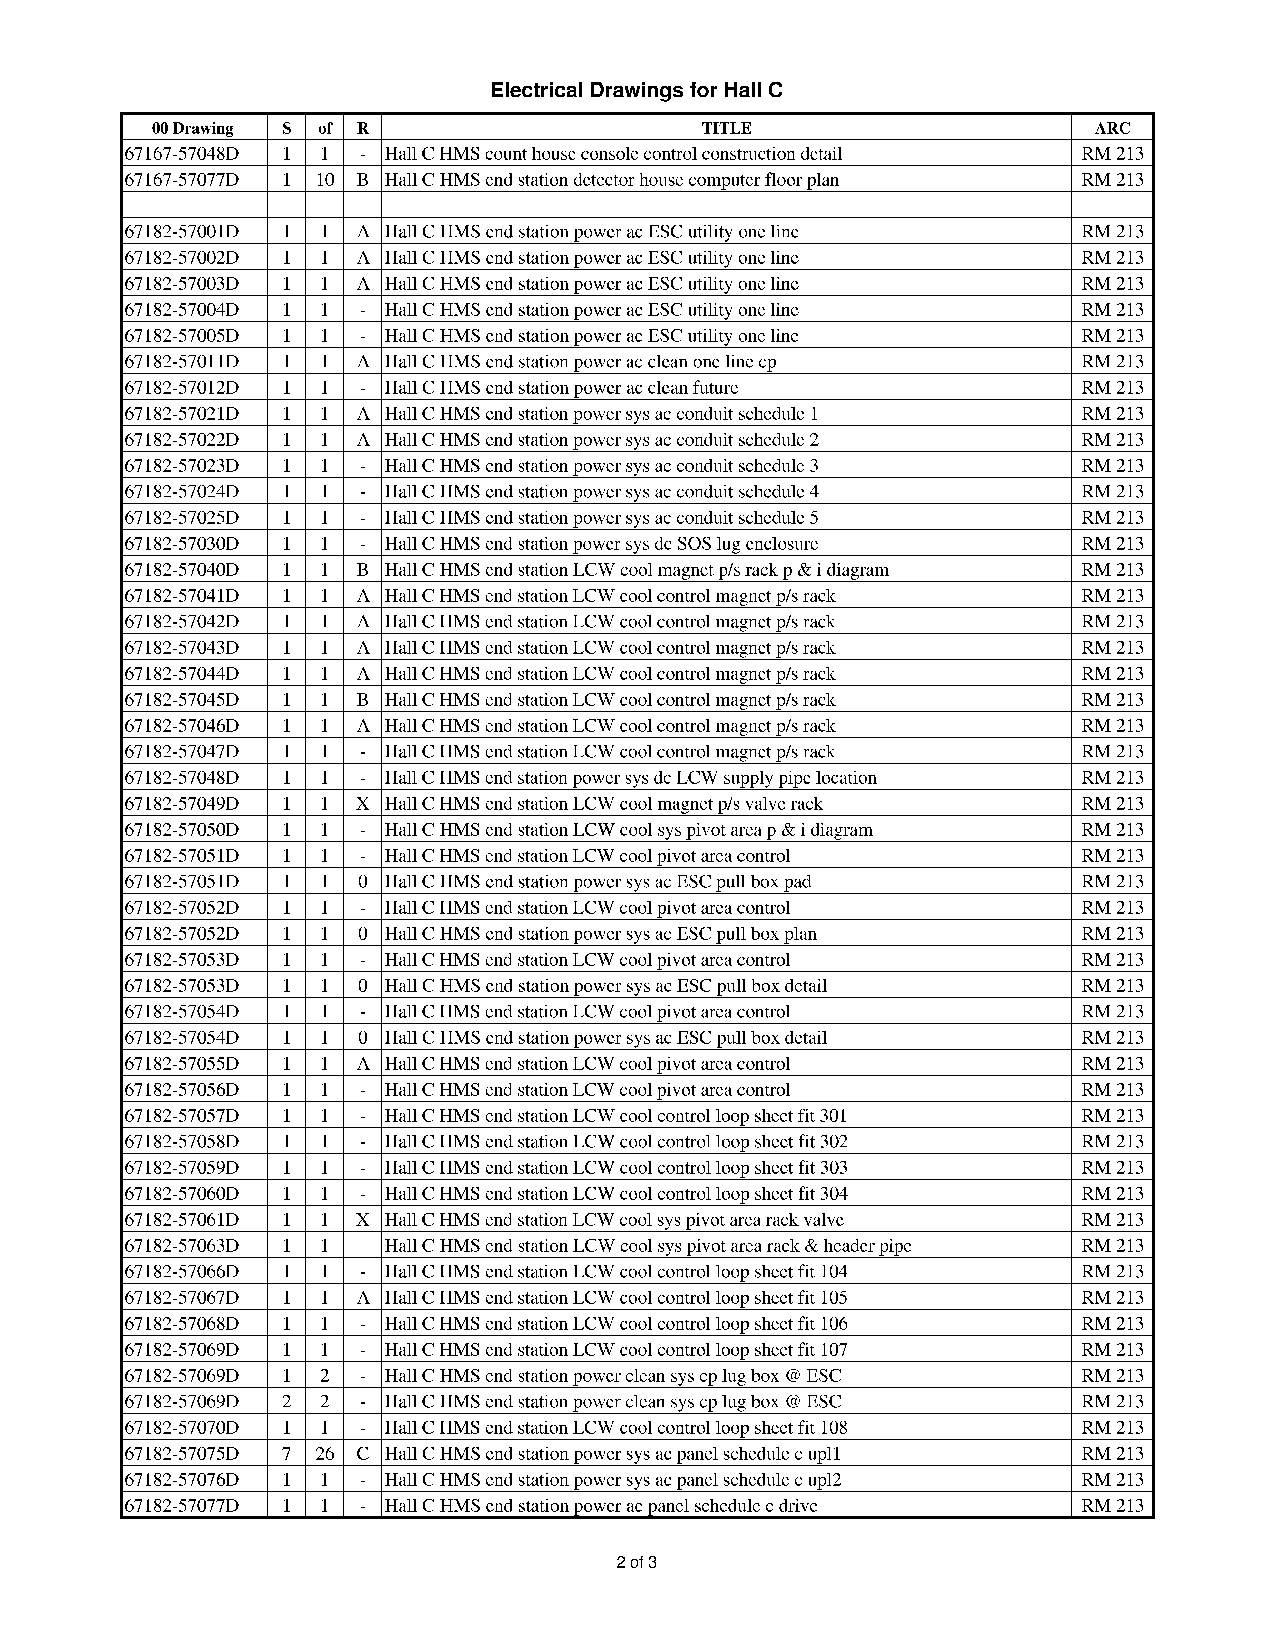
\includegraphics[height=7in]{ele2p.pdf}
\caption{Electrical Drawings for Hall~C (2 of 3)}
\label{fig:elect_dwgs2}
\end{center}
\end{figure}

\clearpage
\begin{figure}
\begin{center}
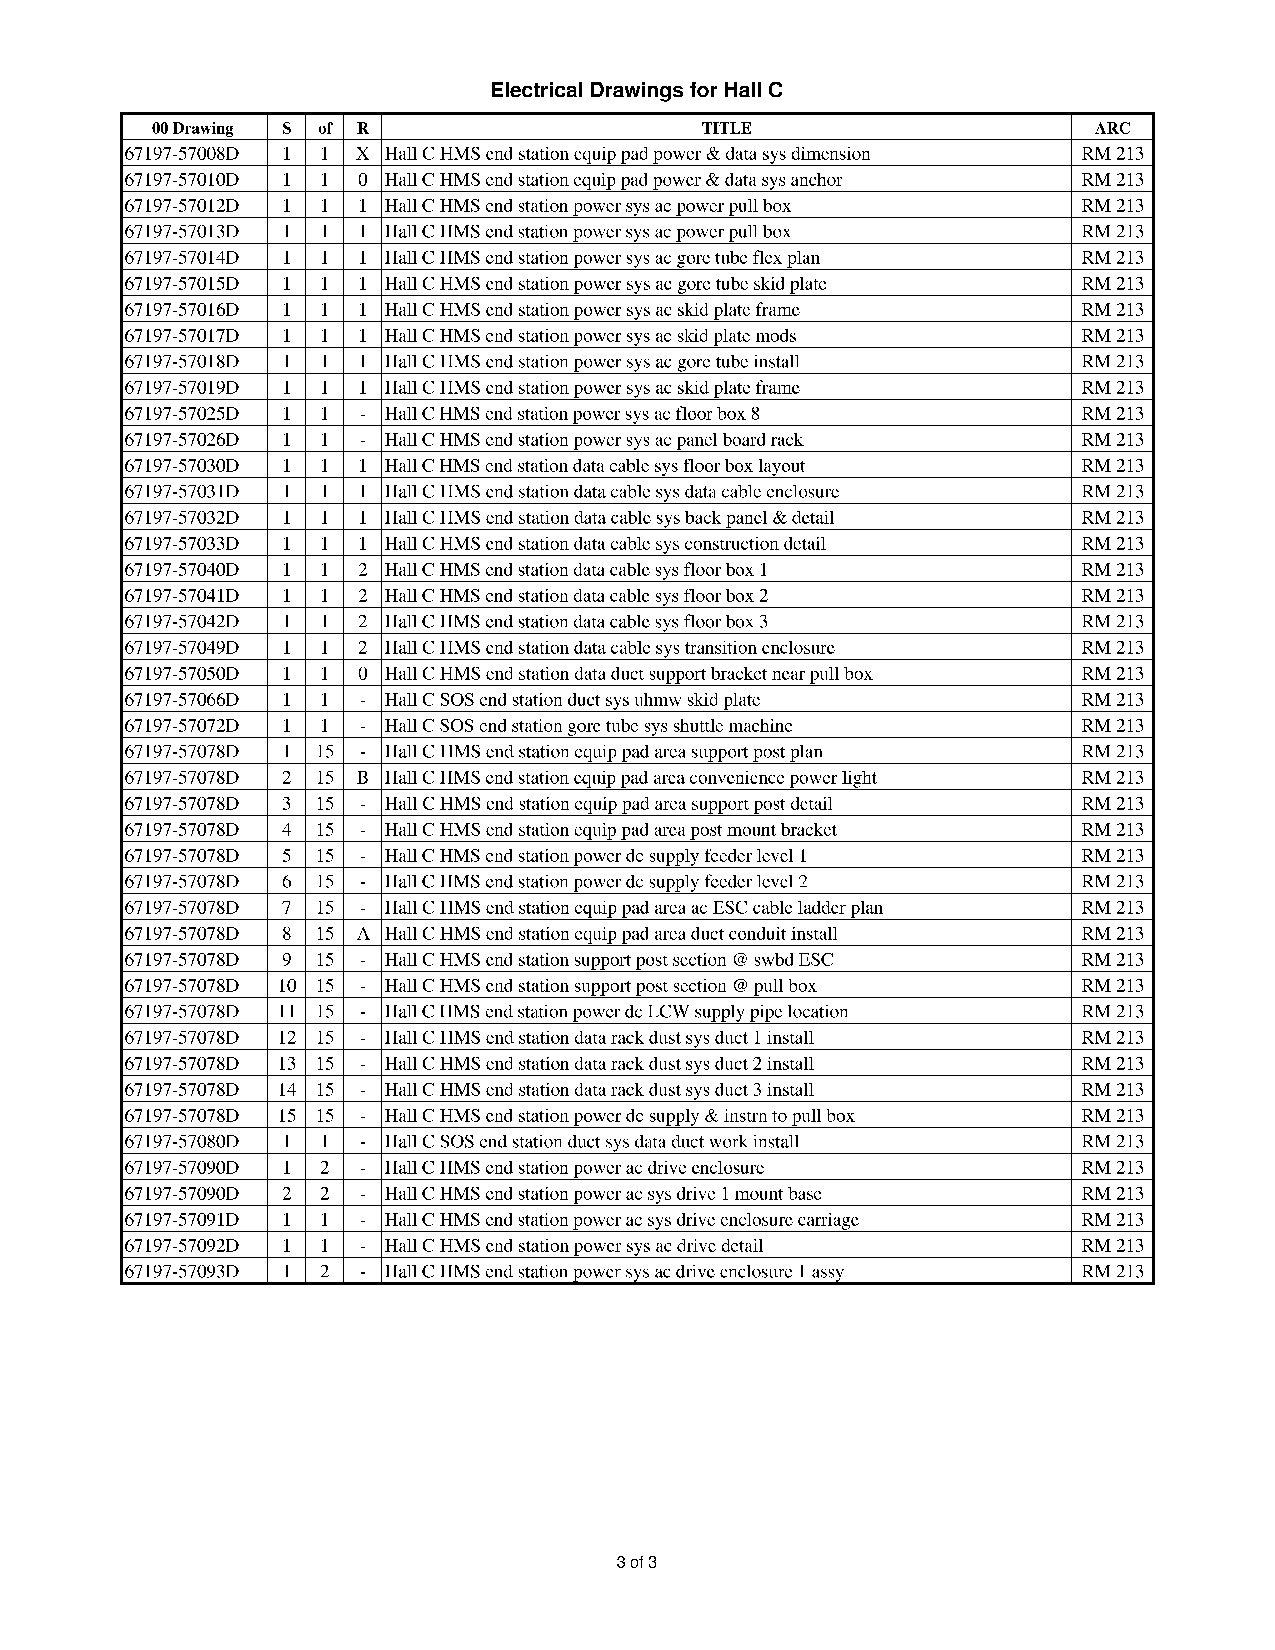
\includegraphics[height=7in]{ele3p.pdf}
\caption{Electrical Drawings for Hall~C (3 of 3)}
\label{fig:elect_dwgs3}
\end{center}
\end{figure}
\clearpage


There are circuit breakers located in several places around Hall~C.
If you encounter equipment that seems unpowered it is always worth checking the
breakers. All outlets in Hall~C  have a label that indicates which
breaker box feeds it. Boxes are located on the north side of the hall behind
the large magnet power supplies, along the side of the SOS and HMS spectrometers
and upstairs in the room next to the Hall C counting room (as you stand outside the
counting house building in front of the door to the Hall~C trigger
room, this room is behind the door to your left). The clean power
breaker is upstairs.

The fire safety (VESDA) system may also be responsible for loss of AC
clean power. For more information see the section on fire in this
manual.

Aside from the resetting of circuit breakers you should not attempt
to solve any problems associated with AC power distribution without
consulting responsible personnel.

{\bf Anyone working on AC power in Hall~C must be familiar with
the EH\&S manual and must contact one of the responsible personnel listed
in the \htmladdnormallinkfoot{ESAD}{http://www.jlab.org/Hall-C/document}}.

\subsubsection{Loss of Site AC Power}

Power failures are unusual but not at all unknown at Jefferson Lab. Typically,
unplanned site-wide power failures occur about once per year. Significant
``glitches'' in the power system are much more common.

If you are working in Hall~C when a power failure occurs, you should
promptly make whatever you are working on safe and exit the hall. Emergency
(power failure) lighting will only last a few minutes. It is designed to
help you safely leave the building. Do not continue working within the
experimental hall during a power failure.

Very few systems in Hall~C will continue to function without AC power. As
necessary for safety, many devices and controls computers are powered through
UPS backups. However, persons working in Hall~C must be aware that not all
systems are on backup power and that there may be significant stored energy
that is not automatically dissipated when AC power is removed. When a 
power outage is planned, there are preparations you can make which will
shorten the time required for recovery. The following paragraphs contain
instructions from the system experts about what to do in advance of, during,
and after a power failure.

\paragraph {System: Cryogenic Target}
(what to do before/during/after a power failure)

\paragraph {System: Vacuum}
(what to do before/during/after a power failure)

\paragraph {System: HMS or SOS Slit Collimators}
After a power cycle the HMS and SOS slits move themselves to the {\it HOME} position,
returning a reading of 0. Thus, after a power failure or other cycle, the slits
must be commanded to a meaningful position using the commands described in
Section~\ref{sssec:slit_control}.
\paragraph {System: HMS and SOS Spectrometers}
(what to do before/during/after a power failure)

\pagebreak[2]
\paragraph {System:M\o ller Polarimeter}~ 

{\bf In preparation for a planned power outage affecting the M\o ller Polarimeter, 
operators should:}

\begin{itemize}
\item Ramp down Q1 and turn off power supply
\item Ramp down Q2 and turn off power supply
\item Put solenoid in non-persistent mode, ramp down, turn off.
\item Move all collimators to RETRACTED position.
\item Move target ladder to RETRACTED position.
\item Depending upon expected duration of power outage:
	\begin{itemize}

   	 \item{more than 5 minutes:}
        Close (0\%) LN2 and LHe supply (JT) valves.
        Close cold return valve.
        Open (100\%) warm return valve.

   	 \item{5 minutes or less:} no change to cryo
	\end{itemize}
\end{itemize}

{\bf Response to an unplanned power failure:}
\begin{itemize}
\item While power is off there is no control nor is there anything
to be controlled. (i.e. there is nothing you can do).

\item Be aware that if the solenoid was ON and in PERSISTENT mode,
it will remain on until the coils warm up from lack of helium.
At that point the magnet will quench, dumping its energy in
the leads and the power supply shunt resistor.

\item Personnel entering the beam tunnel must be aware that the
solenoid field may still be on and that the solenoid is likely
to quench.
\end{itemize}

{\bf Recovery from a power failure (ONLY IF THE M\o ller WAS ON)}
\begin{itemize}
\item (Controls IOCs will normally come up on their own as soon as
power and network communications are available)

\item Re-start vacuum pumps (two of) under the beamline near the
polarimeter. (Also restart other vacuum pumps in the hall related
to cryo transfer lines vacuum.)

\item Contact a M\o ller expert and determine the cryogenic status and
how to proceed. If no expert is available, use the M\o ller cryo MEDM
screen to close LN2 and LHe supply JT valves (if not already closed)
[EV91017 and EV91018], close LHe Cold-Return JT valve [EV91019],
and open warm return ball valve [EV91001]. This will turn off the
cryogen supplies to the M\o ller solenoid.

{\bf NOTE: if the solenoid is still energized (persistent mode) it
is preferable to keep it cold if possible, in order to avoid a
quench.}

\item Using the M\o ller Collimators MEDM screen, execute "GO HOME" on
the target ladder. When the target is HOME execute "GO HOME" on
the collimators. Wait for completion, then send both the target
and the collimators to the RETRACT position unless directed
otherwise by a M\o ller expert.

\item Enter Hall-C and inspect the cooling water flow gauges: make
certain that cooling water is flowing.

\item In the hall, locate the M\o ller controls rack (HC01Z03). Press
"START" on the Q1 power supply. Behind you is the Q2 power supply.
An authorized person should reset it, clear any faults, and return
the supply to REMOTE mode.

\item Notify MCC that the Hall has undergone an interruption of power
and remind them that they must restore the maximum voltage parameter
(known as ``VSET'') on the M\o ller Q1 power supply MEDM screen.

\end{itemize}


\paragraph {System: Beamline Raster}
(what to do before/during/after a power failure)



\subsection{LCW Operations}

Hall~C LCW is controlled at two main locations.  The SOS and M\o ller
polarimeter power supplies are fed from the control rack located next to
the SOS power supplies and are regulated to a pressure of 115 psi.  The
HMS power supplies and SOS magnets are fed from the pivot LCW rack
located near the spectrometer pivot point and operate at line
pressure 200-250 psi.  Return pressure is approximately 50 psi at both
racks and normal supply temperature is usually between 80 and 90 F.

During normal operations the supply, return, and solenoid valves will be
open on all connected circuits.  The green flashing indicators should
light and the flow meters should indicate active lines.  There should be 
no red lights or audible alarms.  
The test circuit and HMS bypass are left closed during
normal operations.

\subsubsection{Loss of site LCW}

If LCW supply pressure drops below approximately 100 psi or LCW flow is
interrupted the low-high pressure and/or low-high flow alarm will sound
and the red indicators begin to flash.  In this event it is recommended
that the shunted test lines on the control racks and the HMS bypass
lines be opened to help mitigate pressure spikes when service is
resumed.  When service is resumed the alarms can be rest by pressing on
the indicator.  If the bypass lines were opened they should be closed at
that time.

\subsubsection{Maintenance}

During maintenance LCW may be shut off to individual branch circuits at
the control racks.  If it is necessary to work on the control racks LCW
may be shut off at the valves located on the north side of the hall
where the main LCW feed and return lines enter.  When shutting down any
LCW circuit branch or main you must close the supply side first (Failure
to do so can trap up to 300 psi in the circuit).  The return side must
also be closed before service to prevent the 50 psi return pressure from
back-feeding the system.  Water (at 50 psi) left in the system can be
drained to the nearest floor drain by attaching a hose to the purge
valves located at the supply and return manifolds, on each control rack.
(The bypass flow alarm on the main console could be set off by this
procedure.  The alarm may be reset as above by pressing the indicator
button after draining is complete.)

Before pressure is reapplied purge valves must be shut.  If the main
supply valves at the wall were closed then the bypass and shunted test
valves should be opened, as for loss of site LCW listed above.  When
applying pressure to the branch circuits the solenoid valves should be
in the open position.  Open the return valve first to bring the system
up to return pressure then slowly open the manual supply valve.  Always
check the system for leaks after any maintenance.


\subsection{Fire}

Because the Ethane used in the wire chambers is a flammable gas
(and due to other fire hazards) a VESDA
system has been installed in Hall~C. There are smoke detectors
for the VESDA system at various places in the hall including in the shield
houses.
The main VESDA panel can be found in the room behind the door at the bottom
of the truck ramp on the left hand side as you walk out of Hall~C. This
panel will indicate where in the Hall the VESDA detected a problem.
A VESDA alarm indicates the possibility of a fire and hence EXTREME caution
should be employed in such an event. It is worth noting that all the
permanent Hall~C staff members have received JLab's fire safety training.

All the detectors in the HMS hut are powered by clean power. The
hut clean power is interlocked to the VESDA system. If the VESDA system
senses smoke, it trips all the clean power in the hut. The sensitivity of the
VESDA head is 0.003 \% to 0.3 \%.

There is a map indicating the evacuation routes of the end station complex
posted outside the Hall~C counting house.

}
